\documentclass[12pt]{article}

\usepackage[utf8]{inputenc}
\usepackage[T1]{fontenc}
\usepackage[brazil]{babel}

\usepackage{geometry}
\geometry{margin=2.5cm}
\usepackage{setspace}
\onehalfspacing

\usepackage{amsmath, amssymb, amsthm}
\usepackage{mathtools}

\numberwithin{equation}{section}

\theoremstyle{plain}
\newtheorem{theorem}{Teorema}
\newtheorem{proposition}[theorem]{Proposição}
\newtheorem{lemma}[theorem]{Lema}
\newtheorem{corollary}[theorem]{Corolário}

\theoremstyle{definition}
\newtheorem{definition}[theorem]{Definição}
\newtheorem{example}[theorem]{Exemplo}
\newtheorem{exercise}{Exercício}

\theoremstyle{remark}
\newtheorem*{remark}{Observação}

\usepackage{csquotes}
\usepackage{xcolor}
\usepackage[colorlinks, citecolor=blue, urlcolor=blue, linkcolor=green]{hyperref}

\usepackage[
    backend=biber,
    style=abnt
]{biblatex}



\addbibresource{../Microeconomics.bib}

\newcommand{\R}{\mathbb{R}}
\newcommand{\pref}{\succeq}
\newcommand{\strictpref}{\succ}
\newcommand{\indiff}{\sim}

% ------------------------------------------------
% Title (fill manually)
% ------------------------------------------------
\title{Lista 1 -- Teoria Microeconômica (PPGE-UFF)}
\author{Professor: Fábio Waltenberg\thanks{\href{mailto:fdwaltenberg@id.uff.br}{fdwaltenberg@id.uff.br}} \\Monitor: Nicholas Funari Voltani\thanks{\href{mailto:nicholasvoltani@gmail.com}{nicholasvoltani@gmail.com}}}
\date{}

\begin{document}

\maketitle

\hypertarget{conceitos-introdutuxf3rios}{%
\section{Conceitos introdutórios}\label{conceitos-introdutuxf3rios}}

\hypertarget{conjuntos-parcialmentetotalmente-ordenados}{%
\subsection{Conjuntos parcialmente/totalmente
ordenados}\label{conjuntos-parcialmentetotalmente-ordenados}}

\begin{definition}[Relações de Ordem]
  Um conjunto (não-vazio) \(X\) é dito \emph{parcialmente ordenado} se ele possui uma relação \(\pref\) que satisfaça\footnote{Note que \(\forall\)   é um ``A'' invertido, que em inglês se lê ``\emph{for \textbf{a}ll}''.
  Por exemplo, a asserção \(\forall x \in X: x \pref x\) lê: ``Para todo
  \(x\) pertencente ao conjunto \(X\), vale que \(x \pref x\)''. Ademais,
  caso valha a asserção lógica \(A \land B\), lê-se: ``\(A\) \textbf{e}
  \(B\) são verdadeiros''.} 
  
  \begin{enumerate}
    \item \emph{Reflexividade}:
\(\forall x \in X: x \pref x\)
    \item \emph{Transitividade}:
\(\forall x, y, z \in X: (x \pref y) \land (y \pref z) \implies x \pref z\)
    \item \emph{Antissimetria}:
\(\forall x, y \in X: (x\pref y) \land (y \pref x) \implies x = y\)
  \end{enumerate}


Essa relação \(\geq\) é dita ser uma \emph{relação de ordem parcial} (ou
relação \emph{parcial} de ordem).

Caso \emph{todos} os elementos em \(X\) sejam ``comparáveis'' através de
\(\pref\) --- ou seja,\footnote{Caso valha a asserção lógica
  \(A \lor B\), lê-se: ``\(A\) \textbf{ou} \(B\) é/são verdadeiro(s)''.
  Note que este ``ou'' é \emph{inclusivo}, ou seja, quer dizer ``\(A\) é
  verdadeiro, \(B\) é verdadeiro, ou \(A\) \textbf{e} \(B\) são
  verdadeiros''.} \[
\forall x, y \in X: (x \pref y) \lor (y \pref x)
\] dizemos que o conjunto \(X\) é \emph{totalmente ordenado}, e que
\(\pref\) é uma relação de ordem \emph{total} (ou relação \emph{total} de
ordem).


\begin{remark}
  
  Note que, naturalmente, nem todas as relações parciais de ordem são
  totais. Seja \(X = \{ 1,2,3\}\), e
\(\mathcal{P}(X) = \{ \emptyset, \{ 1 \}, \{ 2 \}, \{ 3 \}, \{ 1,2 \}, \{ 1,3 \}, \{ 2,3 \}, X \}\)
o conjunto das partes de \(X\) (em inglês: \emph{power set}). Verifique
que \(\mathcal{P}(X)\), com a relação de inclusão de conjuntos
\(\supseteq\), é uma relação \emph{parcial} de ordem, mas que \emph{não
é total} --- ou seja, existem elementos em \(\mathcal{P}(X)\) que não
são comparáveis sob \(\supseteq\).

Para enxergá-lo, pode ser útil ver o diagrama de Hasse deste conjunto, vide abaixo. 

\begin{figure}[h]
  \centering
  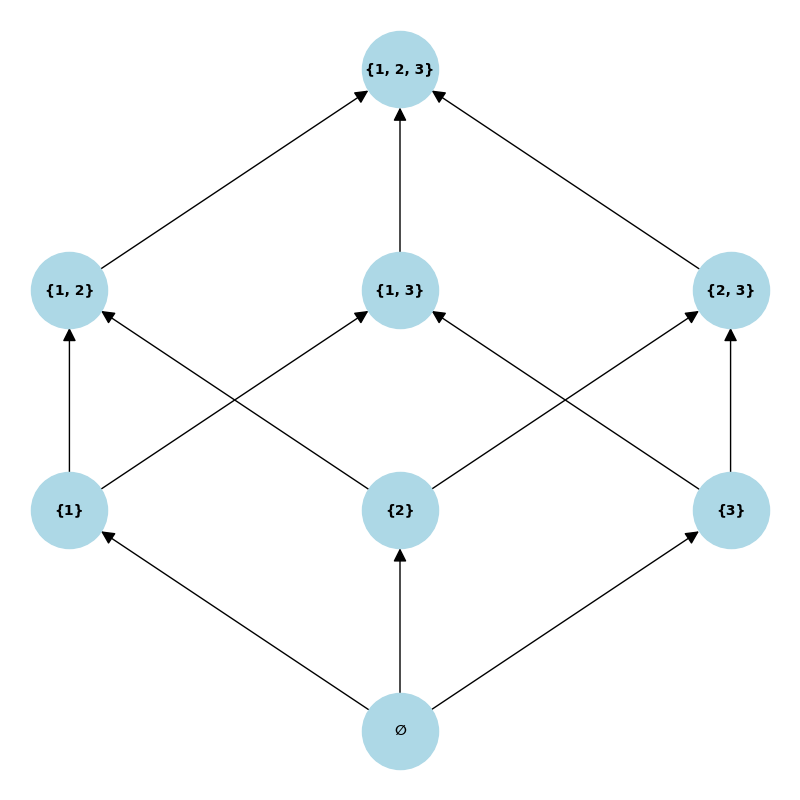
\includegraphics[width=.6\linewidth]{Hasse_diagram.png}
  \caption{Diagrama de Hasse para o conjunto (parcialmente) ordenado $\mathcal{P}(\{1, 2,3\})$ pela relação $\supseteq$. As setas apontam de um ``conjunto-contido'' ao ``conjunto-que-o-contém'': existe a seta $A \to B$ se e somente se $B \supseteq A$ (ou, equivalentemente, $A \subseteq B$).}
\end{figure}

Note-se, pela figura, que o conjunto $\{1\}$ está relacionado a (i.e. contido em) o conjunto $\{1, 3\}$, mas que o conjunto $\{2\}$ não está relacionado com $\{1,3\}$!  

(Ao leitor atencioso: trivialmente pode-se definir \(x \preceq y\) --- a
operação ``para o outro lado'' --- como \(y \succeq x\).)

\end{remark}
\end{definition}

\begin{definition}[Relações de Equivalência]
  Uma relação $\sim$ sobre um conjunto $X$ (não-nulo) é dita ser uma \textit{relação de equivalência} se ela satisfaz as seguintes propriedades:
  \begin{enumerate}
      \item \emph{Reflexividade}: \(\forall x \in X: x \sim x\) [Todo elemento é ``equivalente a si mesmo''.] 
      \item \emph{Comutatividade}: \(\forall x, y \in X: x \sim y \iff y \sim x\) [Ou seja, $x \sim y$ é verdade se, e somente se, $y \sim x$ é verdade. Ambos sempre são verdadeiros juntos, e falsos juntos.]
      \item \emph{Transitividade}: \(\forall x, y, z \in X: (x \sim y) \land (y \sim z) \implies x \sim z\)
    \end{enumerate}
  
  Relações de igualdade são relações de equivalência, mas a recíproca não é verdadeira: há relações de equivalência que não são igualdades. Portanto, falar de equivalência é algo mais geral do que igualdade, i.e. menos restritivo. 

  Um exemplo pode auxiliar: as listas $[1, 2, 3]$ e $[\square, \triangle, \circ]$ não são iguais, porém eu consigo definir uma função bijetiva tal que, por exemplo,
  \[
  \begin{cases}
    1 \mapsto  \circ \\
    2 \mapsto \square \\
    3 \mapsto \triangle
  \end{cases}
  \]
  
  Ela é bijetiva, pois possui a função inversa
  \[
  \begin{cases}
    \square \mapsto  2 \\
    \triangle \mapsto 3 \\
    \circ \mapsto 1
  \end{cases}
  \]
  
  Ou seja, ambos os conjuntos são, de certa forma, equivalentes, pois ``possuem a mesma forma''. Aliás, em Matemática, dizemos que dois conjuntos são \textit{isomorfos} quando há uma bijeção entre eles; essa é uma das formas mais ubíquas de se falar de equivalências em Matemática (mas não a única).

\end{definition}


\hypertarget{preferuxeancias-racionais}{%
\subsection{Preferências racionais}\label{preferuxeancias-racionais}}

\begin{definition}[Preferências Racionais]
  
  \textcite{Mas-Colell1995} definem \emph{preferências racionais} \(\succeq\) como
  ``relações \emph{completas} [\(\forall x,y: (x \succeq y) \lor (y \succeq x)\)] e \emph{transitivas}'' --- ou seja, vide acima, são relações de ordem \emph{total} sobre um espaço de cestas de bens.
\end{definition}

\begin{definition}[Função utilidade representante de preferências racionais]
  
  Vide definição \textbf{1.B.2.} em \textcite{Mas-Colell1995}, uma função
  \(u: X \to \mathbb{R}\) é uma \emph{função utilidade que representa uma
relação de ordem} \(\succeq\) caso \[
  \forall x, y \in X: x \succeq y \iff u(x) \geq u(y)
  \] (naturalmente com a relação de ordem \(\geq\) usual dos números reais
  \(\mathbb{R}\).)
\end{definition}
  

\begin{proposition}
  Todas preferências que sejam representáveis por uma função utilidade são necessariamente racionais.

  \begin{proof}
    A relação de ordem sobre os reais \(\mathbb{R}\) \emph{é uma relação
    total}, pois sabemos que, para quaisquer números reais
    \(x, y \in \mathbb{R}\), vale que ou \(x>y\), ou \(x<y\), ou \(x=y\);
    dito de outra forma, sempre vale que ou \(x \geq y\), ou \(y\geq x\).
      
    Dessa forma, caso uma relação de preferências \(\succeq\), sobre um
    conjunto \(X\) de cestas de bens, seja representável por uma função
    utilidade \(u:X \to \mathbb{R}\), então \emph{necessariamente} esta
    relação tem de ser \emph{racional} (i.e.~relação \emph{total} de ordem).
    A demonstração da proposição \textbf{1.B.2} em \textcite{Mas-Colell1995} segue o
    seguinte esquema: para quaisquer \(x, y \in X\), como \(u(x)\) e
    \(u(y)\) estão sobre um conjunto totalmente ordenado \(\mathbb{R}\),
    então vale que ou \(u(x) \geq u(y)\), ou \(u(y) \geq u(x)\), e como
    pressupõe-se que \(\succeq\) é representada por \(u\), então conclui-se
    que ou \(x \succeq y\) ou \(y \succeq x\) --- portanto, esta relação
    \(\succeq\) é total.
    
    Ou seja, caso uma relação de preferências seja representável por uma
    função utilidade, então ela será racional.
  \end{proof}

  \begin{remark}
    A recíproca não é verdadeira:
    há preferências racionais que não são representáveis por funções
    utilidade, uma das quais é a ordem lexicográfica (exercício \ref{velhojorge} abaixo).    
  \end{remark}
\end{proposition}

\section{Exercícios} 
\setcounter{exercise}{0}
\subsection{Relações de ordem e preferências racionais}
\begin{exercise}
  Dada uma relação de ordem (parcial) \(\succeq\) em um espaço \(X\), defina-se uma relação \(\sim\) em $X$ como \[
  \forall x, y \in X: x \sim y \iff (x \succeq y)\,  \land  \, (y \succeq x)
  \] 
  (Tradução: ``Para todo \(x\) e \(y\) pertencentes a \(X\), vale que \(x \sim y\) se, e somente se, valer que \(x \succeq y\) e também \(y \succeq x\).) 
  
  Demonstre que esta relação $\succeq$ realmente é uma relação de equivalência.  
  
\end{exercise}

\begin{exercise}
  Dada uma relação de equivalência \(\sim\) sobre
algum conjunto (não-vazio) \(X\), então é possível definir, para cada
\(x \in X\), sua \emph{classe de equivalência} \([x]\) como sendo o
conjunto\footnote{Tradução matemática: \([x]\) \emph{é definido} como
  ``o conjunto de elementos \(y \in X\) tais que \(x \sim y\)''. Note
  que estes elementos \(y\) são um mero índice, i.e.~não importa qual
  letra seja usada; poderia igualmente ser escrito como ``o conjunto de
  elementos \(z \in X\)'', ou ``\ldots elementos \(\xi \in X\)''. O
  único elemento que tem alguma ``concretude'' aqui (além do dado
  conjunto \(X\)) é um dado elemento \(x\), que foi pré-determinado no
  enunciado.} \[
[x] \coloneqq \{y \in X: y \sim x\}
\]

Ou seja, é o conjunto de elementos em \(X\) que são equivalentes (sob
\(\sim\)) a \(x\) (note que \(x \in [x]\) --- por quê?).

Demonstre que classes de equivalência são \textbf{disjuntas}: se há
algum elemento em comum entre duas classes de equivalência \([x]\) e
\([y]\), então elas são a mesma classe de equivalência. Em matematiquês:\footnote{\(A \implies B\) lê ``\(A\) implica \(B\)'', ou seja, \(A\)
  ser verdadeiro \emph{implica que} \(B\) também seja verdadeiro.
  \(A \iff B\) quer dizer que \(A\) é verdadeiro \emph{se e somente se}
  \(B\) for verdadeiro; é o mesmo que \(A \implies B\) \textbf{e também}
  \(B \implies A\).}
\[
\forall x, y \in X: \exists z \in [x] \cap [y] \iff [x] = [y]
\]

  Dito de outra forma: vale que $[x] \neq [y]$ se, e somente se, não há interseção entre suas classes de equivalência --- i.e.~\([x] \cap [y] = \emptyset\). Em matematiquês: \[
\forall x, y \in X: [x] \cap [y] = \emptyset \iff [x] \neq [y]
\]


\begin{remark}
  A importância deste exercício é que, dada uma relação de preferência
  racional \(\succeq\) sobre algum conjunto de cestas de bens \(X\), é
  possível definir uma relação de equivalência \(\sim\) , a qual descreve
  uma ``relação de indiferença'' entre cestas de \(X\). As \emph{curvas de
  indiferença} são, portanto, classes de equivalência sob esta relação de
  equivalência induzida por esta preferência. Segue do resultado acima,
  portanto, que \emph{curvas de indiferença diferentes não se cruzam}! Note como este conceito \textbf{não depende de funções utilidade}! 
  \end{remark}
\end{exercise}

\begin{exercise}
  Uma função \(f:X \to Y\) definida
sobre conjuntos parcialmente ordenados \((X, \succeq_{X})\) e
\((Y, \succeq_{Y})\) é dita ser uma função \textit{monotônica} quando ela  \emph{preserva relações de ordem}, i.e. se temos \(x \succeq_{X} x^{\prime} \) em \(X\), então
\(f(x) \succeq_{Y} f(x^{\prime} )\) em \(Y\). Em matematiquês: \[
\forall x, y \in X: x \succeq_{X} x^{\prime}  \implies f(x) \succeq_{Y} f(x^{\prime} )
\]

Mostre que relações de equivalência induzidas por relações de ordem (vide acima) são também preservadas por funções monotônicas \(f\): se \(x \sim_X x^{\prime} \), então
\(f(x) \sim_Y f(x^{\prime} )\).

Isso quer dizer que, embora ``os valores mudem'' por conta da função
\(f\), \emph{o formato das curvas de indiferença permanecem os mesmos}.


\begin{remark}
  É comum se dizer que funções monotônicas são ``funções
  não-decrescentes'', e que funções \emph{estritamente} monotônicas são
  ``funções \emph{estritamente} crescentes'' --- isso, porém, segue da
  definição de acima\footnote{Usualmente também assume-se que o domínio da
    função \(f\) seja \emph{totalmente} ordenado, que é o caso de
    \(\mathbb{R}\): todos os elementos são comparáveis entre si sob a
    relação de ordem. Mas isso é mero pedantismo: se dois elementos
    \(x, y \in X\) não fossem comparáveis sob relação de ordem, então já
    não haveria nada entre eles para ser preservado por \(f\), e tudo se
    passaria como se nada tivesse se passado!}. 
    
Funções monotônicas em
  geral preservam \(\succeq\), mas pode haver casos em que, por exemplo,
  \(x \succ_{X} x^{\prime} \) \textbf{e} \(\mathbf{x \nsim_{X} x^{\prime} }\), mas
  \(f(x) \succeq_{Y} f(x^{\prime} )\), ou até \(f(x) \sim_{Y} f(x^{\prime} )\) --- por
  exemplo, funções em \(\mathbb{R}\) que sejam crescentes mas que possuam
  ``platôs'' nos quais certos intervalos estejam ``na mesma altura'' num
  gráfico; são, portanto, funções ``não-decrescentes''. 
  
  Por outro lado,
  funções \emph{estritamente} monotônicas preservam somente \(\succ\) ---
  se \(x \succ_{X} x^{\prime} \), então garante-se que \(f(x) \succ_{Y} f(x^{\prime} )\) ---
  e, portanto, são funções \emph{estritamente} crescentes.
  \end{remark}
\end{exercise}

\begin{exercise}
  Considere uma relação de preferência definida
  sobre \(\mathbb{R}^2\) definida como \[
  (x_{1},x_{2}) \succ (y_{1}, y_{2}) \iff x_{1}+x_{2} < y_{1}+y_{2}
  \]
  
  Essa relação de preferência satisfaz não-saciedade local? Há algum ponto de saciedade local? 
\end{exercise}


\begin{exercise}
  \label{velhojorge}
  A ordem lexicográfica \(\succeq\) é uma relação
  de ordem definida para quaisquer \(x=(x_{1},x_{2}) \in \mathbb{R}^{2}\)
  e \(y =(y_{1},y_{2})\in \mathbb{R}^{2}\) como \[
  x \succeq y \iff (x_{1} \geq y_{1}) \lor [(x_{1} = y_{1}) \land (x_{2} \geq y_{2})]
  \] É chamada ``lexicográfica'', pois é um ordenamento ``alfabético'': por
  exemplo, \(ab \succeq aa\), pois \(a=a\) (ou seja, \(x_{1}=y_{1}\)) e
  \(b\geq a\) (ou seja, \(x_{2}\geq y_{2}\)).
  
  Em outras notícias, o velho Jorge tem problemas com bebida. Seus amigos falam em voz baixa sobre suas curvas de nível lexicográficas: ele sempre prefere estritamente a cesta de consumo que contém a maior quantidade de bebida, independentemente da quantidade dos outros bens na cesta; se duas cestas tiverem a mesma quantidade de bebida, ele prefere estritamente a cesta que tem a maior quantidade dos outros bens. Esboce as preferências do
  velho Jorge em um diagrama. Elas satisfazem completude e transitividade? Ela é uma relação de ordem \emph{contínua}? 

\end{exercise}  

\section{Resoluções}
\setcounter{exercise}{0}

\begin{exercise}
      Para ser uma relação de equivalência, a relação \(\sim\) acima definida deve satisfazer as propriedades: 
    \begin{enumerate}
      \item \emph{Reflexividade}: Seja $x \in X$. Então $x \sim x$ é o mesmo que dizer $(x \succeq x) \land (x \succeq x)$. Como $\succeq$ é uma relação de ordem, então ela satisfaz que, para qualquer $x$, $x \succeq x$. Portanto, a asserção $x \sim x$ é verdadeira.
      
      \item \emph{Comutatividade}: Sejam $x, y \in X$. Então $x \sim y$ é o mesmo que $(x \succeq y)\,  \land  \, (y \succeq x)$, o que é o mesmo que (invertendo os argumentos) $(y \succeq x)\,  \land  \, (x \succeq y)$ --- que é o mesmo que $y \sim x$. Portanto, $x \sim y$ é equivalente a $y \sim x$.
      
      \item \emph{Transitividade}: Sejam \( x, y, z \in X\) tais que \((x \sim y) \land (y \sim z)\). Então vale que (já reescrevendo-o de maneira sugestiva)
      \[
      \underbrace{ (x \succeq y) \land  (y \succeq z) }_{ \iff x \succeq z } \land \underbrace{ (z \succeq y) \land (y \succeq x) }_{ \iff z \succeq x }
      \]
      Portanto, vale que $(x\pref y) \land (y \pref x) \implies x = y$.
    \end{enumerate}
  
    Por satisfazer estas propriedades, \(\sim\) é, de fato, uma \emph{relação de equivalência}.

\end{exercise}


\begin{exercise}
  $(\impliedby)$ Isso é trivial, pois, caso os conjuntos $[x]$ e $[y]$ sejam os mesmos, qualquer elemento deles estará na interseção --- afinal, são o mesmo conjunto!

  $(\implies)$ Tenha-se, por exemplo, $z \in [x] \cap [y]$; ou seja, $z \in [x]$ e $z \in [y]$. Vale, em particular, que $z \sim x$ e $z \sim y$. Queremos demonstrar que $[x] = [y]$, ou seja, que vale $[x] \subseteq [y]$ --- ou seja, $\forall x^{\prime} \in [x]: x^{\prime} \in [y]$ --- e também $[y] \subseteq [x]$. 

  $(\subseteq)$: Seja $x^{\prime} \in [x]$. Então, como $x^{\prime} \sim z$ --- pois ambos pertencem a $[x]$ ---, e $z \in [y]$, então $x^{\prime} \sim y$ --- portanto, $x^{\prime}  \in [y]$. Logo, como $\forall x^{\prime} \in [x]: x^{\prime} \in [y]$\footnote{Pois $x^{\prime}$ foi um elemento arbitrário escolhido em $[x]$.}, provou-se que $[x] \subseteq [y]$.
  
  $(\supseteq)$: Seja $y{\prime} \in [y]$. Então, como $y^{\prime} \sim z$ --- pois ambos pertencem a $[y]$ ---, e $z \in [x]$, então $y^{\prime} \sim x$ --- portanto, $y^{\prime} \in [x]$. Logo, como $\forall y^{\prime} \in [y]: y^{\prime} \in [x]$, provou-se que $[y] \subseteq [x]$.
  
  Portanto, conclui-se que, caso $[x] \cap [y] \neq \emptyset$, então $[x] = [y]$.

  Note que o argumento de que classes de equivalência sem interseção são classes distintas segue a mesma ideia: se não há elemento algum na interseção entre $[x]$ e $[y]$, então não há nenhum elemento que permita a ``ponte'' entre elas. \textbf{Esse} é o centro da argumentação da demonstração acima!  
\end{exercise}

\begin{exercise}
  Temos que, pelo exercício anterior,
  \[
  x \sim_X x' \iff (x \pref_X x^{\prime})  \land (x^{\prime} \pref_X x)
  \]
  
  Logo, como $f$ é monotônica, teremos que 
  \[
  \begin{cases}
  x  \succeq_{X} x^{\prime}  \implies f(x) \succeq_{Y} f(x^{\prime} ) \\
  x^{\prime} \succeq_X x \implies f(x^{\prime} ) \succeq_Y f(x)
  \end{cases}
  \]

  Portanto, vale que 
  \[
  x \sim_X x^{\prime}  \implies f(x) \sim_Y f(x^{\prime} )
  \]
\end{exercise}

\begin{exercise}
 O ponto $y = (0, 0)$ é um ponto de saciedade local, pois não há nenhum outro ponto ``menos preferível'' do que ele. 
\end{exercise}

\begin{exercise}
  A ordem lexicográfica satisfaz completude --- todos os pontos são relacionáveis entre si, herdado das relações de ordem em $\mathbb{R}$ em cada dimensão $x$ e $y$ ---, e transitiva.
  
  Ela não satisfaz continuidade: seja $(x_n)$ uma sequência de números $x_n > 0$ para todo $n$, tais que $x_n \to \infty $ conforme $n \to \infty$. Então temos que os pontos 
  \[(x_n, 0) \pref (0, 1)
  \]
  pois $x_n > 0$, e, portanto, o limite
  \[
  \lim\limits_{n \to \infty} (x_n, 0) \to (0, 0)
  \]
  Note, porém, que, como o limite é do tipo $x_n \to 0^+$ (i.e. se aproximando pelo lado positivo), temos que, para cada $x_n$, $(x_n, 0) \pref (0, 1)$; \textbf{contudo}, o valor do limite em si, $(0, 0)$ não é preferível a $(0, 1)$.  
  
  Escrito de forma mais sugestiva, 
  \[
  \underbrace{ \lim\limits_{n \to \infty} \pref\left((x_n, 0), (0, 1)\right) }_{ \text{Verdadeiro} } \neq \, \underbrace{ \pref\left(\lim\limits_{n \to \infty} (x_n, 0), (0, 1)\right) }_{ \text{Falso} }
  \]
  Portanto, temos que $\pref$ não preserva o resultado deste limite. Logo, $\pref$ não é contínua. 

\end{exercise}

\printbibliography

\end{document}
